\begin{table}[H]
    \centering
    \hspace*{-1.75cm}
    \begin{tabular}{rc|c|>{\centering\arraybackslash}p{0.5\linewidth}|} 
        \cline{3-4} 
        & Fallabbildung & Bedingungen & Bewertung \\\cline{3-4}
        \vspace{-1.35em} \\ \cline{3-4}
            1&\begin{minipage}{0.25\textwidth}
                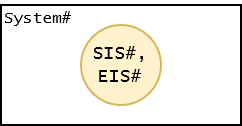
\includegraphics[width=\linewidth]{gfx/IA_1.drawio.png} 
            \end{minipage}
            &$\begin{array}{l}
                \scriptstyle EIS\# \;=\; SIS\#; \\
                \scriptstyle EIS\#,\; SIS\# \;\subseteq\; System\#
              \end{array}$ 
            &\begin{minipage}{0.5\textwidth} 
                \smaller
                \textit{Optimalfall}: Geschätzte Betroffenheit beschränkt sich auf die beschriebene Änderung.
            \end{minipage} 
            \\ \cline{3-4}
            2&\begin{minipage}{0.25\textwidth}
                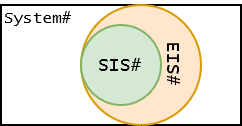
\includegraphics[width=\linewidth]{gfx/IA2.drawio.png} 
            \end{minipage}
            &$\begin{array}{l}
                \scriptstyle |EIS\#| \;>\; |SIS\#|; \\
                \scriptstyle SIS\# \;\subset\; EIS\#; \\
                \scriptstyle EIS\#,\; SIS\# \;\subseteq\; System\#
              \end{array}$ 
            & \begin{minipage}{0.5\textwidth} 
                \smaller
                \textit{Erwarteter Fall}: Die Analyse hat einige wenige Entitäten bestimmt, welche nicht in der primären Änderungsdefinition enthalten sind.
            \end{minipage} 
            \\ \cline{3-4}
            3&\begin{minipage}{0.25\textwidth}
                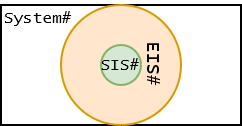
\includegraphics[width=\linewidth]{gfx/IA3.drawio.png} 
            \end{minipage}
            &$\begin{array}{l}
                \scriptstyle |EIS\#|\; \gg \; |SIS\#|; \\
                \scriptstyle SIS\# \;\subset\; EIS\#; \\
                \scriptstyle EIS\#,\; SIS\# \;\subseteq\; System\#
              \end{array}$ 
            & \begin{minipage}{0.5\textwidth}
                \smaller
                \textit{Suboptimal}: Eine große Diskrepanz zwischen \acsfont{SIS\#} und \acsfont{EIS\#} bedeutet einen höheren Arbeitsaufwand in späteren Schritten oder einer schlechten primären Änderungsdefinition.
            \end{minipage} 
            \\ \cline{3-4}
        \cline{3-4}
    \end{tabular}
    \caption{Mögliche \acsfont{SIS\#}/\acsfont{EIS\#} Abhängigkeiten nach Arnold et al. \cite[297]{app_bohner}}
    [Eigene Darstellungen]
    \label{tab:sis_eis}
\end{table}
